%# -*- coding: utf-8-unix -*-
%%==================================================
%% chapter01.tex for SJTU Master Thesis
%%==================================================

%\bibliographystyle{sjtu2}%[此处用于每章都生产参考文献]
\chapter{绪论}
\label{chap:intro0}

\section{自动语音识别}
\label{chap:intro0-asr}


在日常生活中,语音是人与人之间交流最主要也是最有效方式。目前人机交互方式主要由键盘、鼠标和触摸屏来完成,随着移动设备的不断发展,过去的人机交互方式已经不再适用。用语音来进行人机交互能极大提高移动设备的易用性。使用语音来进行人机交互包含语音识别、语义理解、对话管理和语音合成等关键技术,而其中自动语音识别(Automatic Speech Recognition, ASR)作为整个闭环的入口无疑是最重要一环。它的功能就是将人的语音转换为相应文本或者指令以用于后续的处理。

\subsection{语音识别简史}
\label{chap:intro0-asr-history}


最早的语音识别系统出现在1952年贝尔实验室~\cite{davis1952automatic},这是一个只能进行孤立数字识别的系统。它没有使用通用计算机和任何统计机器学习的方法,只是一个精心设计端到端电路。现代的语音识别的基础开始于70年代,代表是隐马尔可夫(Hidden Markov Model, HMM)模型提出~\cite{baker1975dragon, jelinek1976continuous}。在这个模型中,观测特征的生成过程可以被两个条件概率所描述,发声的过程被描述为一个随机生成过程:状态转移概率和状态输出概率。HMM被用来对发声单元进行建模,发声单元包括音素,词或者句子。
在接下来的几十年中,随着高斯混合模型(GMM)被用于模拟状态输出概率和GMM-HMM理论的不断发展以及计算资源的不断改进,语音识别得到了显着的发展。语音识别任务也从简单的孤立词识别任务发展到大词汇量连续语音识别任务。从1988年开始,美国国家标准与技术研究所(National Institute of Standards and Technology, NIST)以及美国国防部高级研究计划局(Defence Advanced Research Project Agency, DARPA)联合组织几场对连续词汇语音识别评估。
这些评估极大地推动了语音识别研究的发展,并为语音识别设定了几个里程碑。语音识别词汇从1988年的资源管理任务中的900个单词改进到1993年华尔街日报中的20000个单词,实现了真正的词汇连续语音识别。不仅词汇量增加,而且语音识别的任务也朝着更现实的识别任务发展。例如,记录环境从干净的环境变为嘈杂的环境,并且记录工具从专用记录设备变为普通电话语音。随着记录环境变得更加复杂,优化的目标也从孤立的单词变为连续的单词序列预测。在20世纪90年代后期,在HMM的基础上,研究人员进一步提出了自适应和自适应训练技术~\cite{anastasakos1996compact,digalakis1995speaker,furui1989unsupervised,gales1998cluster,gales1998maximum,gales2001adaptive,gales2001multiple,gauvain1994maximum,kuhn1998eigenvoices,lee1996speaker,leggetter1995maximum,neumeyer1995comparative,pye1997experiments}来应对不断复杂的语音环境,以及序列鉴别性训练技术~\cite{bahl1986maximum,schluter2001comparison,chou1993minimum,goel2000minimum,juang1997minimum,povey2005discriminative,povey2001improved}来使用序列级准则进行模型优化。这两项技术是在深度神经网络(Deep Neural Network, DNN)提出之前对GMM-HMM系统在复杂环境下提升性能最核心的技术。苹果手机第一代Siri中使用的就是这些技术。

最早在20世纪90年代~\cite{bourlard1989continuous,bourlard1992cdnn,bourlard2012connectionist},研究人员提出了一种使用神经网络(NN)对隐马尔可夫模型中的状态输出概率进行建模的方法。但是,由于当时缺乏计算资源和数据,该框架没有达到比GMM-HMM系统更好的性能。随着摩尔定律继续有效,今天的计算机计算能力已经从二十年前实现了巨大的飞跃。通用图形处理单元(GPGPU)使计算机能够更快地执行并行计算,从而可以训练更强大的模型。随着越来越先进的移动互联网和云计算,现在可以更轻松地收集足够的训练数据。这些因素都使得深度神经网络(Deep Neural Network, DNN)在今天可以被成功地训练。DNN-HMM提出是对GMM-HMM框架的一次变革,令语音识别性能再次获得了巨大的提高,真正走出了实验室研究层次~\cite{ASRBook-Yu2014,CD-DNN-HMM-dahl2012,DNN4ASR-hinton2012,qian2016very,TDNN-peddinti2015,Deepspeech2-amodei2015,LACE-yu2016,xiong2017microsoft}。谷歌、微软、苹果等国际IT巨头近年都推出了以语音识别为核心技术的商业级产品。


字错误率(WER)是衡量语音识别系统质量的重要指标。给定正确注释和语音识别系统的解码结果,将单词错误率定义为两个单词序列之间的编辑距离,值越小越好。图~\ref{fig:WER}反映是截止到2009年深度神经网络出来之前NIST赞助的各个语音识别任务词错误率变迁。其中横坐标是时间,纵坐标是词错误率,每一条折线代表着一项语音识别任务。
\begin{figure}[!htp]
  \centering
    \captionstyle{\centering}
    \centering
    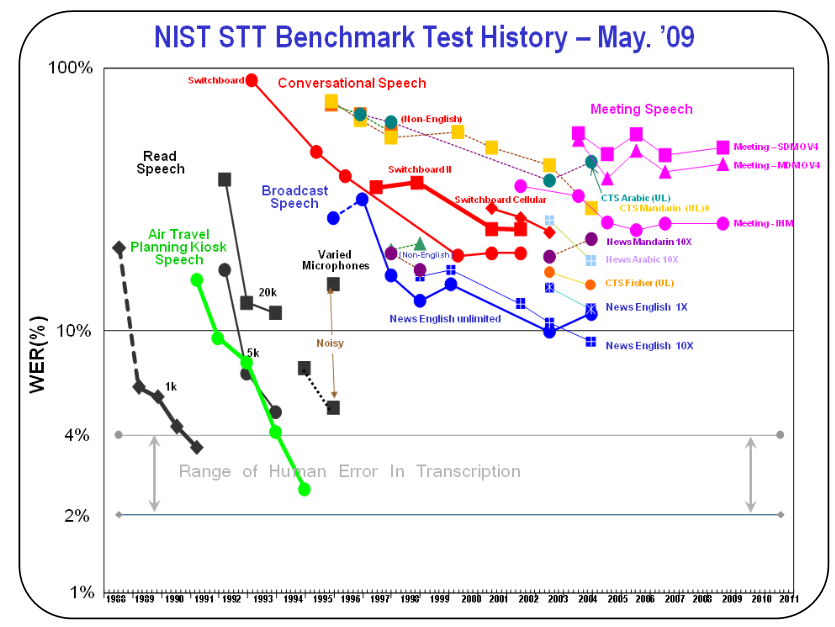
\includegraphics[width=.7\textwidth]{WER.png}
    \bicaption[fig:WER]{}{语音识别词错误率变迁图(截止2009年)}{Fig}{History of WER on several tasks (until 2009)}
\end{figure}

最早的任务是在干净的环境中阅读语音识别。随着GMM-HMM模型的改进与人类的识别率相同,到了20世纪90年代,任务逐渐接近日益复杂的现实环境。仅使用GMM-HMM模型,单词错误仍然很高。其中一个标志性的任务是Switchboard,它是一种电话语音识别。语音识别任务中最大的两个困难是:第一,语音信号是高度非线性信号;第二,声学环境(扬声器,噪声等)对语音信号有很大影响。从图中可以看出,任务场景越向右开,就越难。在21世纪初,学者们分别研究了判别训练和自适应方法来解决这两个问题。可以看出,Switchboard的字板错误率已大大降低。2010年,微软学者提出使用深度神经网络对语音信号进行建模。神经网络的高非线性与语音信号非常吻合,并且Switchboard字的错误率进一步降低。由于DNN-HMM框架是GMM-HMM框架的一次革命,序列识别训练和自适应技术是独立于框架的两个技术方向。因此,他们在新框架下有了新的发展空间。近年来,基于深度神经网络序列的判别训练和自适应技术已成为新时代语音识别领域的核心研究内容。本文主要研究基于深度神经网络的自适应技术。


\subsection{语音识别架构}
\label{chap:intro0-asr-framework}


在迄今为止最为成功的基于统计的语音识别框架中,语音识别过程可以被抽象为如下数学公式:

\begin{equation}
    \label{eq:asr}
    \mathbf{w}^* = \arg \max_{\mathbf{w} \in \mathcal{H}}P(\mathbf{w}|\mathbf{O})
\end{equation}

即在所有可能的候选假设$\mathcal{H}$中寻找拥有最大后验概率$P(\mathbf{w}|\mathbf{O})$词序列$\mathbf{w}^*$。其中$\mathbf{w}=\left[ w_1, ..., w_n \right]$是词序列,$\mathbf{O}=\left[ \mathbf{o}_1, ..., \mathbf{o}_T \right]$是特征向量序列。

\begin{eqnarray*}
    \centering
    \mathbf{w}^* &=& \arg \max_{\mathbf{w} \in \mathcal{H}}P(\mathbf{w}|\mathbf{O}) \\
    &=& \arg \max_{\mathbf{w} \in \mathcal{H}} \frac{p(\mathbf{O}|\mathbf{w})P(\mathbf{w})}{p(\mathbf{O})} \\
    &\propto& \arg \max_{\mathbf{w} \in \mathcal{H}} p(\mathbf{O}|\mathbf{w})P(\mathbf{w}) \\
\end{eqnarray*}

直接对后验概率$P(\mathbf{w}|\mathbf{O})$建模是比较困难的,这个问题可以通过贝叶斯公式转换成条件似然$p(\mathbf{O}|\mathbf{w})$,先验$P(\mathbf{w})$和$p(\mathbf{O})$。因为边缘分布$p(\mathbf{O})$在解码过程中与假设词无关,所以可以忽略掉。在剩下部分中,$p(\mathbf{O}|\mathbf{w})$被称为声学模型,$P(\mathbf{w})$被称为语言模型。声学模型用做建模子词单元生成特征序列的概率的,语言模型描述的是局部语法和整句的语言语义信息。

\begin{figure}[!htp]
  \centering
    \captionstyle{\centering}
    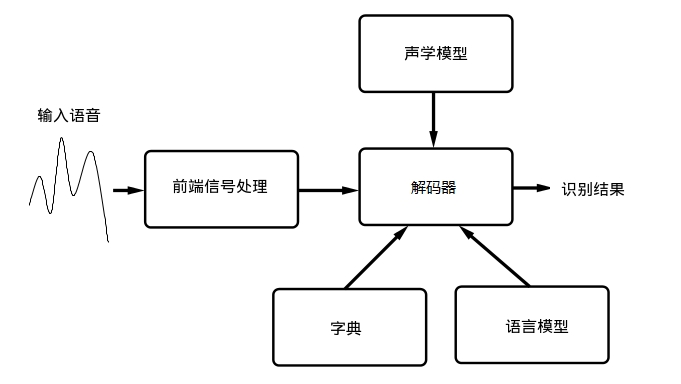
\includegraphics[width=.9\textwidth]{asr.png}
    \bicaption[fig:asr]{}{语音识别框架}{Fig}{Framework of an automatic speech recognition system}
\end{figure}

图~\ref{fig:asr}是对当前流行语音识别系统的框架描述,它主要由四个部分组成,包括前端信号处理、声学模型、语言模型和解码器。
\begin{itemize}
    \item 前端信号处理:原始模拟信号首先由输入设备转换为数字信号。前端信号处理部分负责从数字化语音中提取鲁棒声学特征信息,主要包括多麦克风阵列噪声降低和人耳听觉声学特性的提取。详细内容将在章节~\ref{sec:feat_extra}中介绍。
    \item 声学模型(Acoustic Model, AM): 声学模型是语音识别系统中最重要的模型之一。声学模型的好坏可以直接决定了语音识别系统的性能,也是本论文研究重点之一。声学模型建模的是给定词序列生成出来的所观测到的特征向量序列条件概率$p(\mathbf{O}|\mathbf{w})$,目前主流的语音识别系统通常是使用隐马尔可夫模型(Hidden Markov Model, HMM)来做为声学模型的。在HMM中,存在一个概率分布熵被称为状态输出概率,这个概率可以通过去使用混合高斯模型来得到建模,也可以通过深度神经网络来建模。使用前者语音识别系统可以被称为GMM-HMM系统,使用后者被称为DNN-HMM系统。具体内容将在章节~\ref{sec:hmm}和章节~\ref{sec:dnn_hmm}中详细介绍。
    \item 语言模型(Language Model, LM): 过去了数十年,N元组模型(n-gram)是最主要的使用语言模型~\cite{good1953population,katz1987estimation,brown1992class}。近几年,基于深度神经网络语言模型也逐渐开始得到发展并取得了巨大性能的提升~\cite{mikolov2010recurrent,mikolov2012statistical}。
    \item 解码器及搜索(Decoder): 解码器功能是对声学模型中计算出的声学特征上的概率和语言模型计算出的语言概率去进行组合来得到最大概率的词序列。目前主流的解码算法是去使用基于动态规划思想的维特比算法(Viterbi Algorithm),将在~\ref{sec:decode}和~\ref{chap:intro-lvcsr}中详细介绍。
\end{itemize}

\section{自动语音识别的推理问题}
\label{chap:intro0-inf}

语音识别技术虽然相比多年以前已经有了长足的进步,但是在实际应用中还有很多困难需要处理。其中一个最主要难题就是语音识别推理问题。

%TODO1: 做什么事情
语音识别既是模式识别问题又是相应的推理问题。前一个问题在数学上表示和描述了各种语音和语言现象,并且基于统计学习模式识别框架执行建模,该框架确定了语音识别系统可以实现的识别准确度的上限。在给定模型的情况下,后一问题研究如何使输入语音与模型匹配并推断最佳识别结果,其确定识别速度和实际可达到的识别准确度。在语音识别的推理阶段,解码器功能组合声学模型以计算声学特征概率和语言模型计算的语言概率以获得最大概率词序列。
在语音识别推理阶段,解码器是语音识别系统的核心和灵魂,所有信息都收集在这里。它将来自不同来源,不同层次和不同性质的知识和信息联系起来,以便它们相互补充并获得正确的语音识别结果。因此,如何有机地整合各种不同的信息是解码网络和解码算法设计中必须仔细研究和解决的问题。
从解码器功能的角度来说,它不仅是语音识别研究中各种理论,模型和算法的验证。
正确性和准确性的基本实验平台也是构建实际系统的基础所在。因此,在解码器的设计中必须平衡研究的便利性和工程的实际应用。


%TODO3: 近来深度学习下发展现状和缺陷
近年来,深度学习模型被引入到语音识别声学和语言建模中以取代传统的分类器,显着提高了模式识别问题的准确性。基于深度学习语音识别,语音识别的推理问题没有根本改变,因为它只是取代了分类器。
基于加权有限状态机(WFST)的推理问题静态搜索空间构造技术~\cite{mohri2002weighted}和帧同步维特比(Viterbi)网络搜索算法~\cite{forney1973viterbi}是目前性能最好解决方案,但其仍存在一系列显著缺陷:
\begin{enumerate}
\item 该方案基于传统的混合高斯 - 隐马尔可夫模型(GMM-HMM)声学模型和N-gram语言模型。基于深度学习的声学模型和语言模型是最佳表现。研究还不充分,如何将新的声学和语言模型引入框架; 如何在提高推理速度的同时充分利用模型性能; 如何基于多个知识源给出可靠的推理置信度算法是一个亟待解决的问题。
\item 这种方案基于语音识别中每个知识源(声学,语言,语义等)的搜索空间的预构建和整体优化,产生巨大的搜索空间,包括离线构建,在线使用,动态修改和算法的其他方面。计算量和内存消耗量非常大,这是阻碍语音识别应用场景扩展的重要原因。为了解决这个问题,新的声学和语音模型的搜索空间整体优化是不够的,基于推理中间状态的搜索空间动态优化研究几乎是空白。
\item 目前,语音识别系统基于多知识源建模结果,并对输入音频进行推理。建模和推理过程非常复杂,知识来源的划分依赖于强大的先验知识。大规模或非标记语音数据收集以及基于并行的深度学习技术使得构建直接模拟语音数据和文本序列的端到端模型及其相应的识别和推理算法成为可能。当前的解码框架没有这种设计。
\end{enumerate}

因此,尽管基于深度学习模型,加权有限状态机和基于帧的维特比网络搜索算法的深度学习已经发展到基本可用水平,但是精度仍然不能满足人类之间的正常交流要求。速度限制也使得无法在低成本和低功耗的解决方案上工作,这些解决方案一起阻碍了语音识别技术的大规模商业应用。


\section{论文主要内容、创新点及组织结构}
\label{chap:intro0-thesis}
本论文围绕基于深度序列模型解码搜索技术展开了一系列探索和研究,主要涉及
了基于GPU并行计算的搜索速度优化,基于标签同步解码搜索空间优化,基于标签同步解码的统一解码框架,关键词检测序列建模和标签同步解码等内容。

\begin{enumerate}
    \item 
本论文提出并行的解码搜索算法并在GPU上实现开源该套算法。该框架可以显著加速现有推理算法,特别是在基于深度序列学习一系列模型上进行了验证。

这是一个通用的离线解码器,该解码器对语言模型和声学模型没有特别限制,并且可以工作在各种架构的GPU上。
为了支持第二遍重打分和更丰富后处理,本论文的设计基于WFST解码和词图生成架构~\cite{povey2012generating}。
针对设计中的几大难点,本论文提出了如下解决方案:
本论文将维特比算法中令牌合并操作实现为一个GPU并行计算中的原子操作,以便减少维特比束剪枝算法中同步消耗;本论文提出了动态负载均衡方式以更高效地进行并行计算,提高其多线程之间的利用率;本论文重新设计了基于GPU并行计算精确的词图生成和剪枝算法,以便充分利用GPU性能特点。

在Switchboard 上实验表明,本论文所提出方法在取得完全一致的1-best和词图质量情况下,可以得到3-15倍加速,并在绝大部分GPU架构上进行了验证。除此之外,如果再进行多句子的并行处理,最终加速比将达到46倍。
同时本论文对这项工作进行了开源~\footnote{\url{https://github.com/chenzhehuai/kaldi/tree/gpu-decoder}},
它将与大多数Kaldi脚本相兼容。这项工作作为Kaldi工具包的一个扩展~\cite{povey2011kaldi},完整实现了基于GPU并行计算WFST解码。

\item 本论文基于端到端建模,系统地提出了标签同步算法,其通过一系列方法使得搜索解码过程从逐帧同步变为标签同步,这包括使用高效的blank结构和后处理方法。该文提出一系列通用方法在隐马尔科夫模型和连接时序模型上得到了验证。同时本论文还介绍了将标签同步算法应用于序列到序列的端到端模型方案,使之取得了更快和更好的模型收敛和模型准确度。

具体来说,本论文提出将特征层面搜索过程改变为标签层面,即搜索空间是由不同历史的标签组成,使得解码速率等于标注速率,从而小于特征速率。具体来说,在标签推理阶段,对帧层面声学模型的输出增加一步后处理过程:i)判断当前帧是否存在标签输出;ii)若有,执行搜索过程;若无,则丢弃标签输出。因此该后处理过程可被看作是每个输出标签概率计算近似。与传统方法相比,该方法的优势是搜索空间更小,且搜索过程被大大加速。
本论文提出一系列通用方法在隐马尔科夫模型和连接时序模型上得到了验证。
%
同时本论文还研究了将标签同步算法应用于序列到序列的端到端模型方案。本论文使用模块化训练的思想来改善端到端模型建模,使其更易于使用外在知识源来训练每一个端到端模型子模块。值得注意的是,模型最后需要进行联合优化,因此最终在推理阶段,模型仍然工作在端到端模式下。

在实验部分,本论文提出系统一方面取得大幅度语音识别解码速度改善,另一方面在端到端建模上取得了更快和更好的模型收敛和模型准确度。

\item 本论文提出一系列针对不同应用通用置信度,并尝试将不同应用中的语音识别推理过程统一到同一框架中。

在前面提出标签同步解码算法的基础上,本论文进一步提出了两种置信度生成算法。更细致研究显示这种基于CTC的音素词图是得到更好性能关键所在。
在英文Switchboard 上的大词汇连续语音识别任务显示这里提出LSD CTC 词图置信度算法可以显著改善原先传统的基于逐帧解码算法CTC置信度或者 HMM模型的置信度。
%
另一方面本论文提出一系列针对不同应用通用置信度,并尝试将不同应用中的语音识别推理过程统一到同一框架中。
%
具体来说,本论文提出了辅助归一化搜索空间概念。本论文尝试使用这样的搜索空间来建模所有ASR应用领域置信度。 % and CM can be obtained in an unified framework
而针对这样做在低功耗设备上带来的挑战,本论文采用基于CTC标签同步解码\cite{Chen+2016} 来进行处理,由此带来了很大的效率改善。
最终这一统一高效置信度框架被应用于目前主流的多种ASR应用。

\item 
本论文为深度学习声学非固定关键词的关键词检测设计了相应的序列鉴别性训练方法,同时该方法也可以应用到固定关键词的关键词检测中。

关于如何对序列概率进行定义,可分为序列条件似然度和序列后验概率,这包括两种序列模型: {\em 生成式序列模型} (GSM),比如HMM, 和 {\em 鉴别式序列模型} (DSM),比如 CTC。
对这两种框架,竞争可能性的建模都是核心难题。本论文提出两种方法来解决这一问题:隐性使用音素或半词单元的语言模型来建模,或者显性加入非关键词的标签。

总结本论文的主要贡献包括:
i) 针对生成式序列模型和鉴别式序列模型的序列鉴别性训练的第一个系统研究工作
ii) 提出了一些新颖的办法来构建声学KWS的竞争可能性,以用于鉴别性训练。这些方法显著提升了关键词检测系统的性能。
iii) 基于 LSD框架提出了高效的后处理方法,以便对音素混淆性进行建模。
\end{enumerate}

本文剩余章节安排如下:首先,第\ref{chap:intro}章中将介绍语音识别基本内容;随后,第\ref{chap:intro2}章中会介绍基于深度神经网络自动语音识别,特别是深度序列模型,端到端建模及其在鲁棒语音识别中的应用;继而,第\ref{chap:gpu}章将提出并行解码搜索算法并在GPU上实现开源该套算法;第
\ref{chap:lsd}章基于端到端建模,系统地提出了标签同步算法;第\ref{chap:unify}章提出将不同应用中语音识别推理过程和置信度统一到同一框架中;第\ref{chap:kws}章系统地提出针对深度序列模型的序列鉴别性训练框架;最后,第\ref{chap:sum}章给出本文总结以及对今后可能有用研究思路和展望。
